


\begin{figure}[!h]
\centering
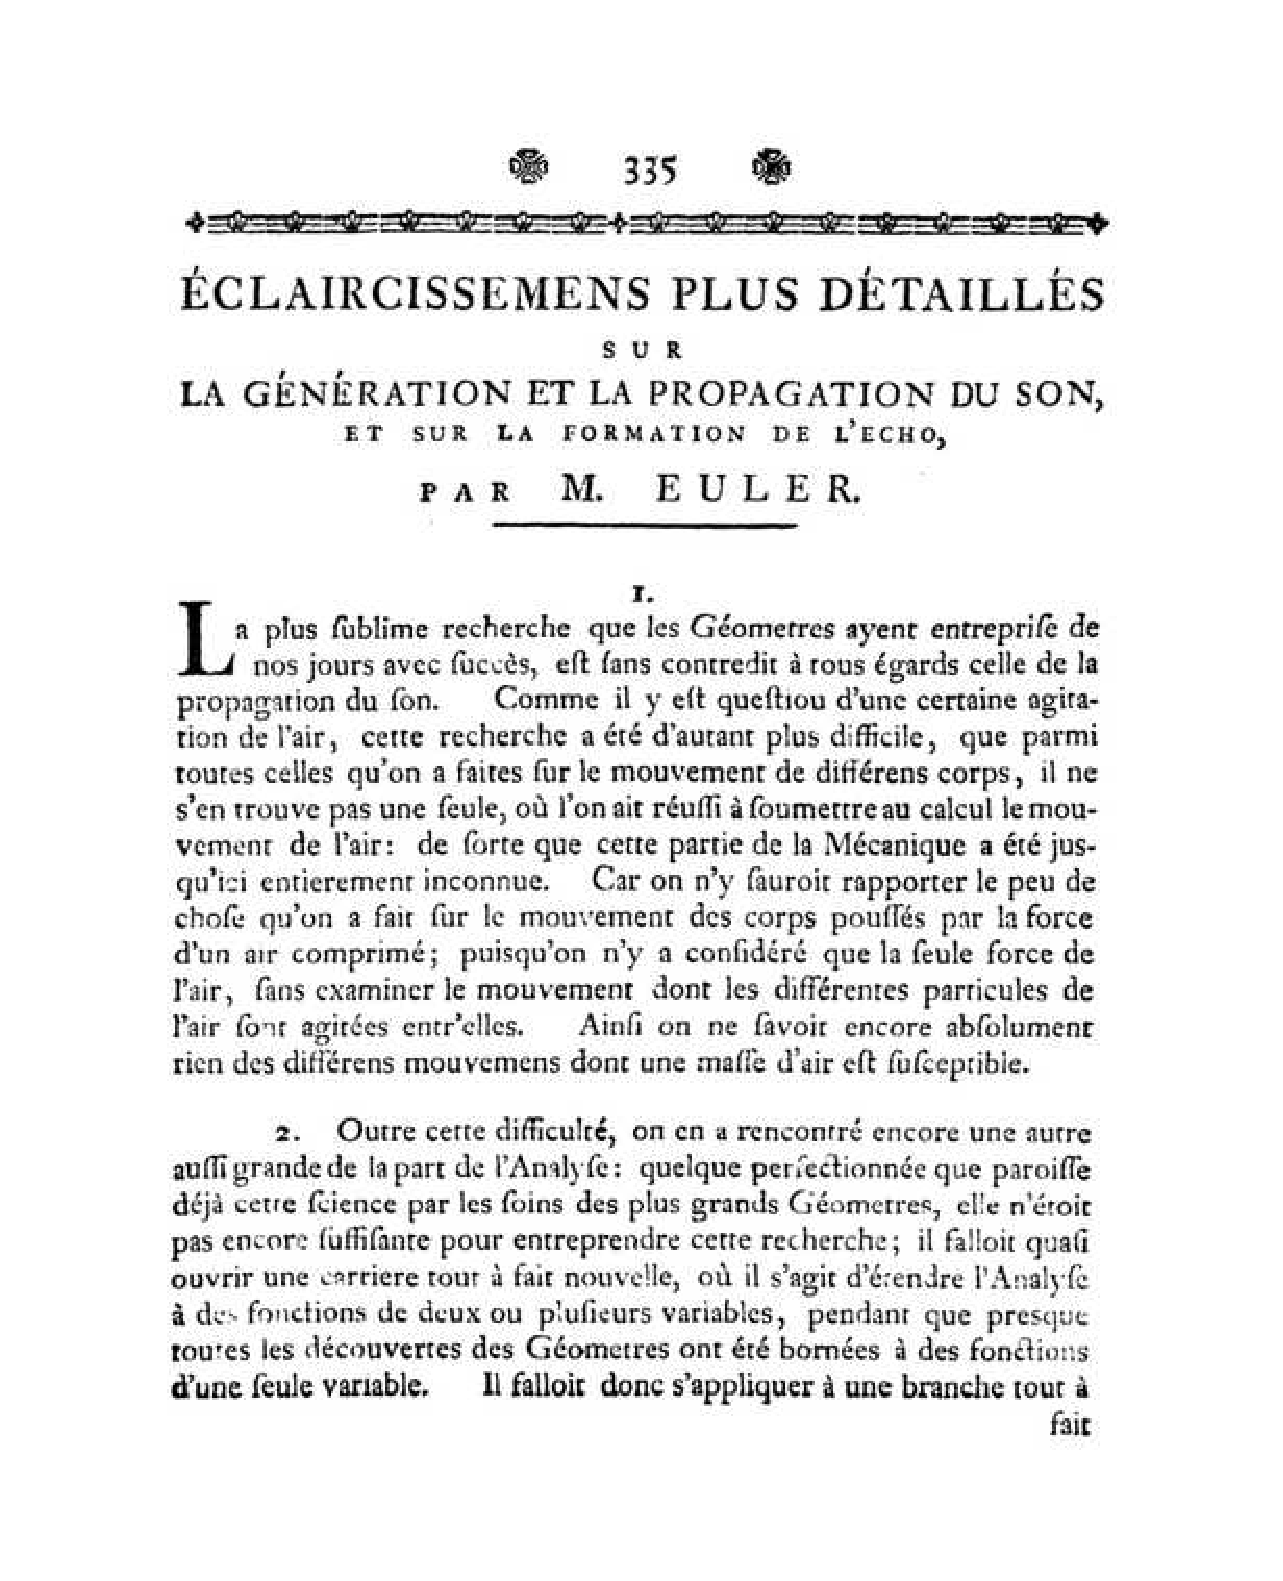
\includegraphics[trim=0.0cm 2.0cm 0.0cm 2.0cm,clip,scale=0.63]{Euler/Euler_p1_1765.eps}

\hspace{-1.3cm}
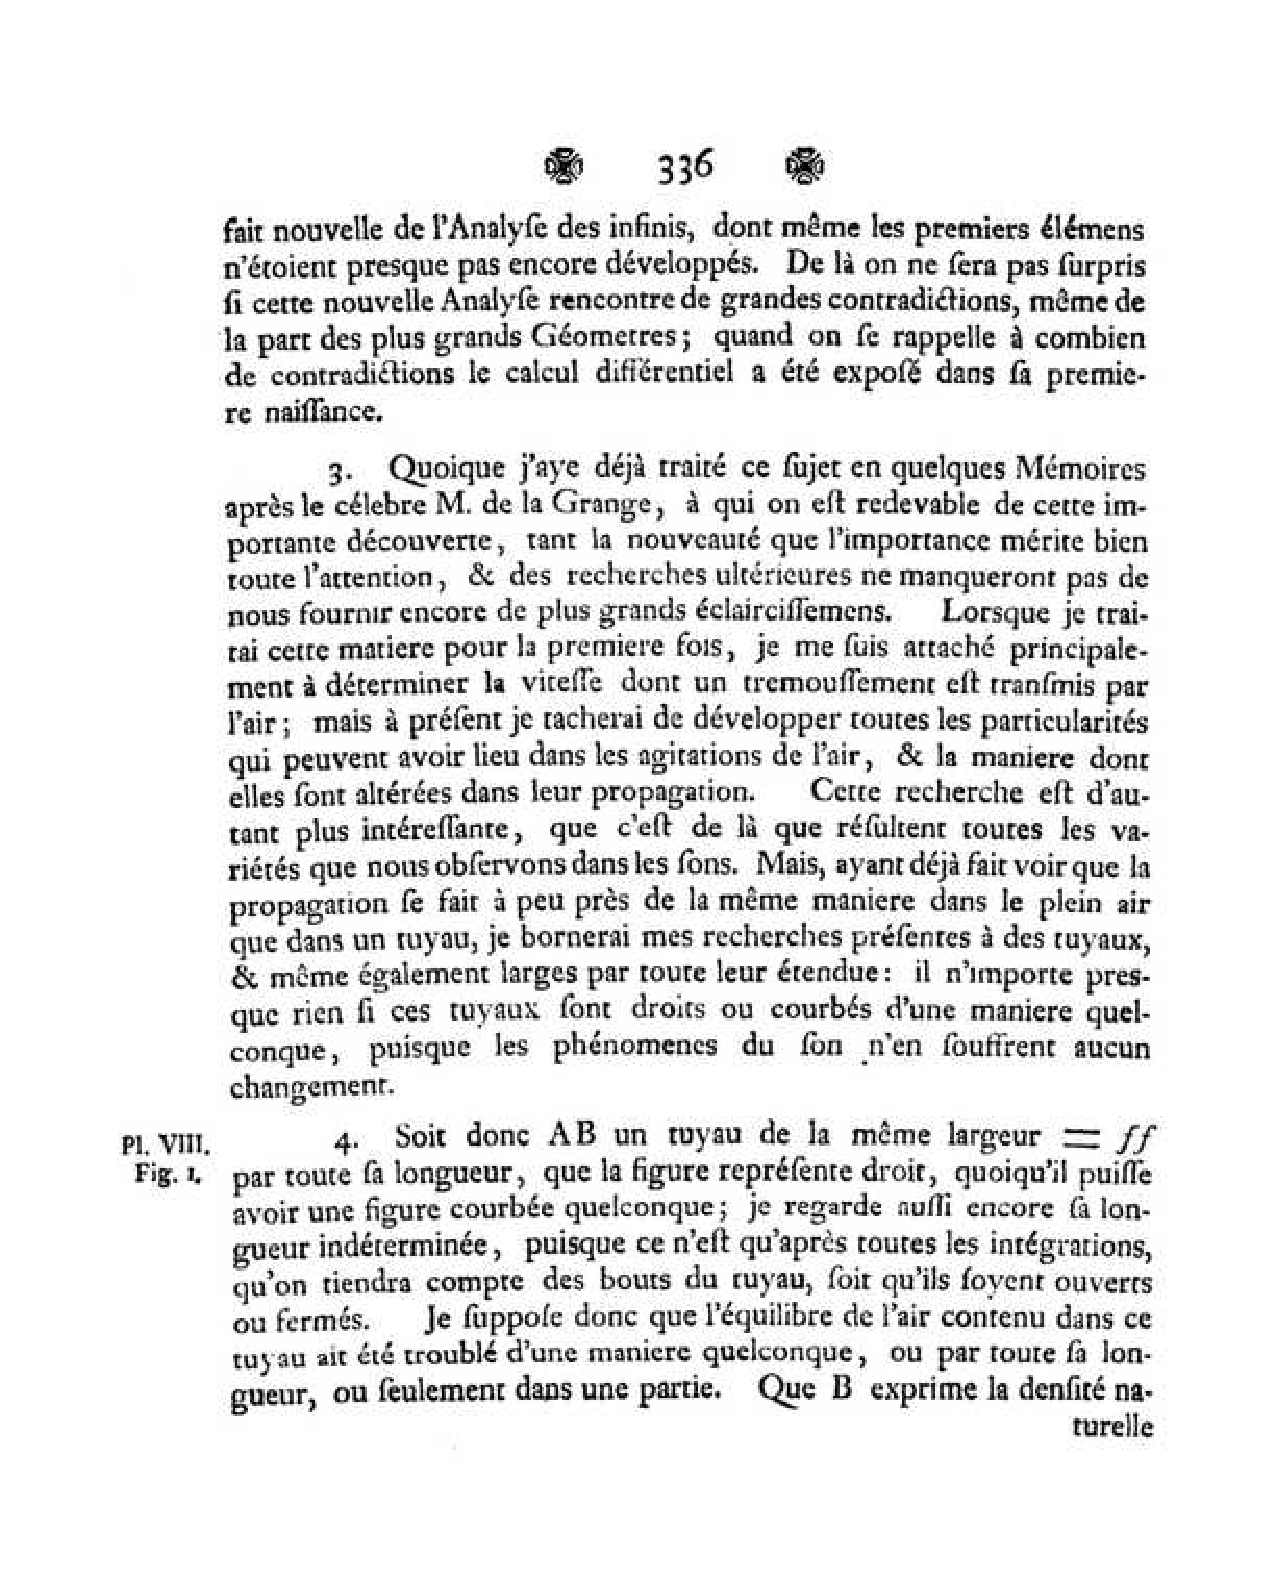
\includegraphics[trim=0.0cm 7.6cm 0.0cm 2.0cm,clip,scale=0.63,angle=-0.5]{Euler/Euler_p2_1765.eps}
\end{figure}

\begin{figure}[!h]
\centering
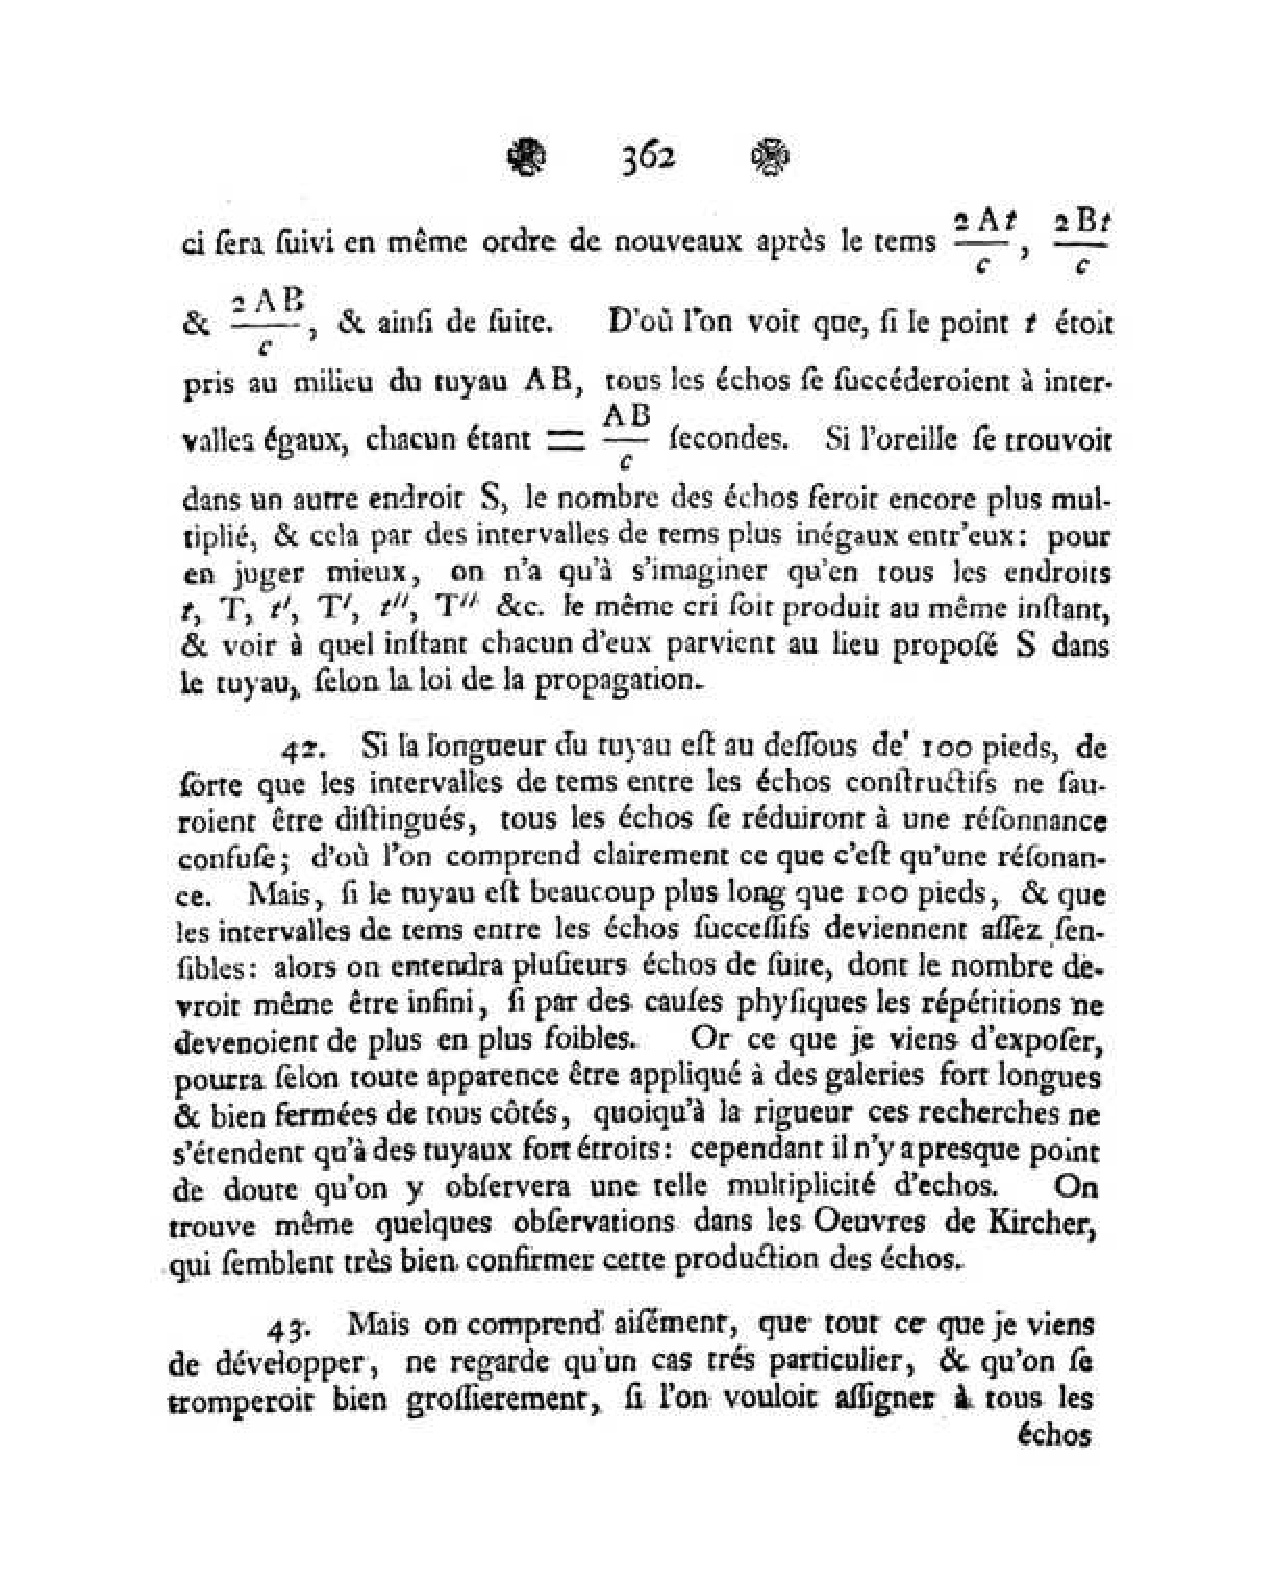
\includegraphics[trim=0.0cm 1.5cm 0.0cm 21.45cm,clip,scale=0.63]{Euler/Euler_p28_1765.eps}

\hspace{-0.5cm}
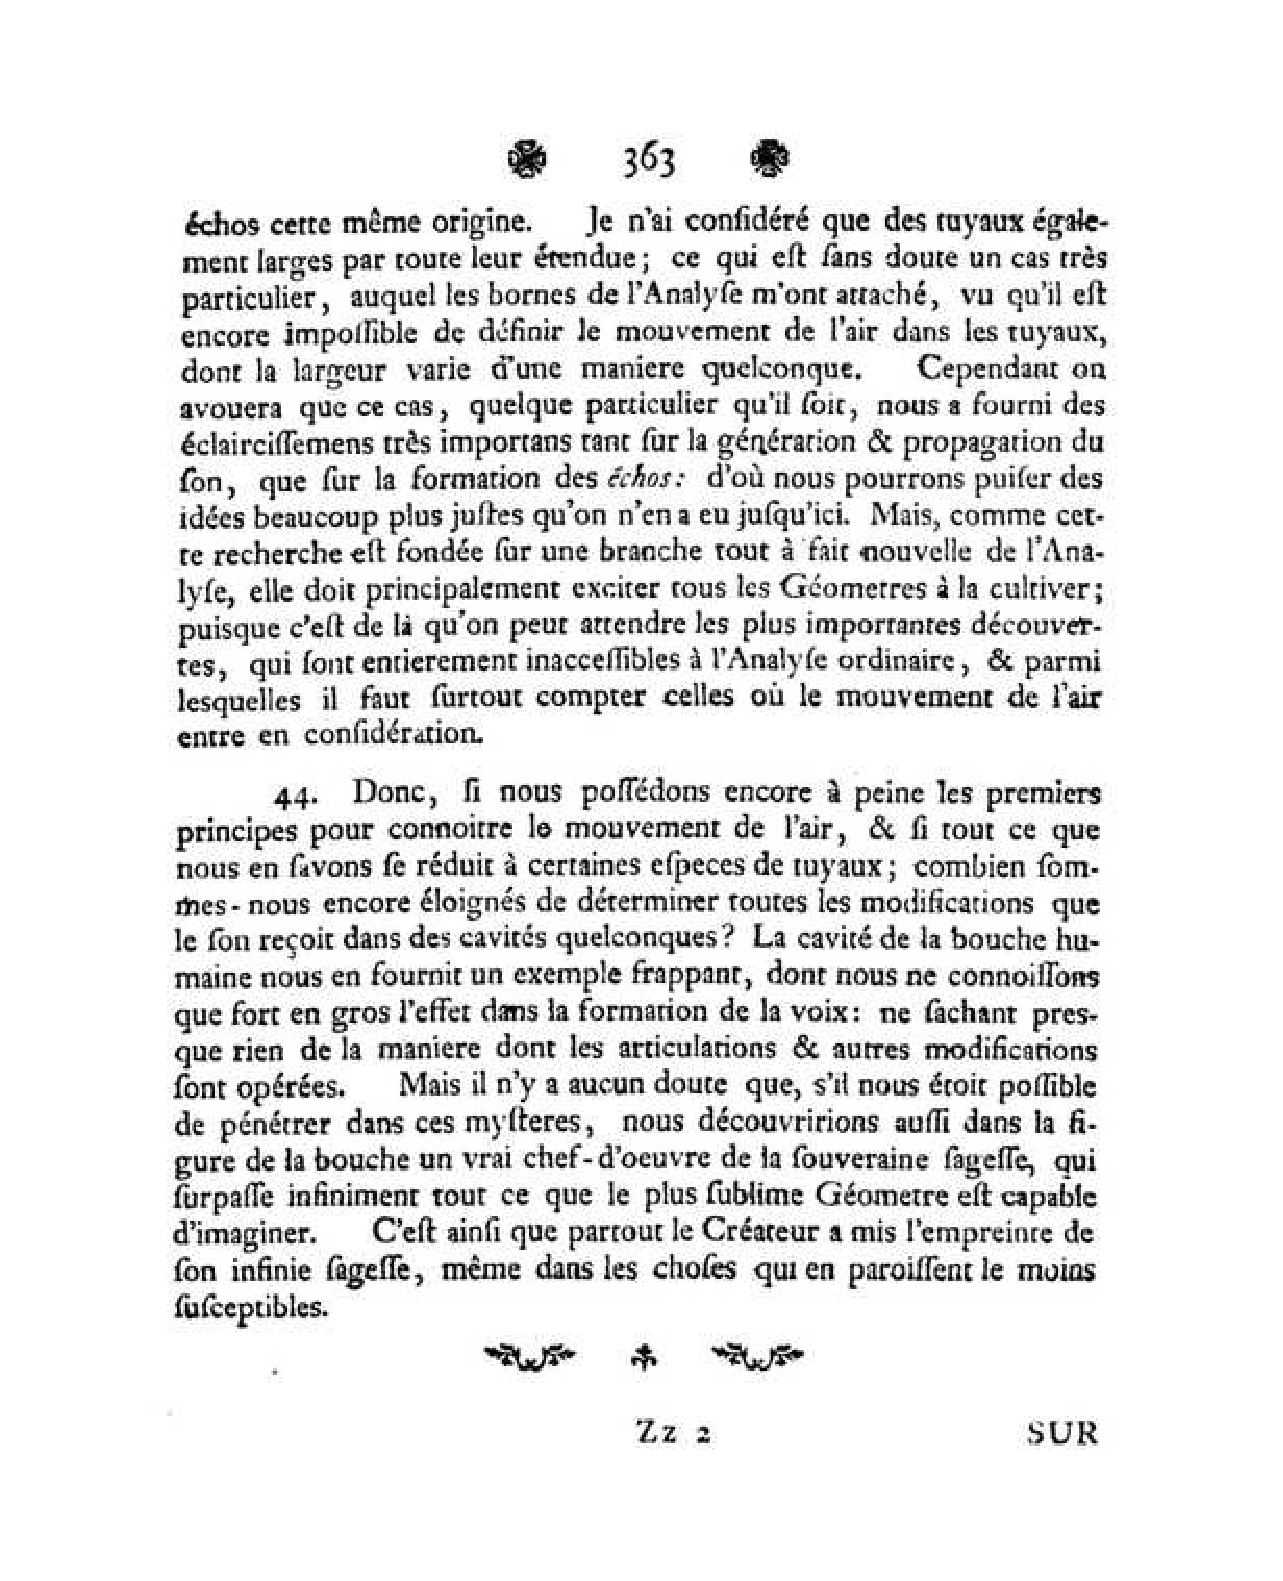
\includegraphics[trim=0.0cm 1.0cm 0.0cm 2.0cm,clip,scale=0.63,angle=0.2]{Euler/Euler_p30_1765.eps}
\caption*{The beginning and ending of the last of Euler's \citeyearpar{Euler_1767} many studies that he contributed on sound propagation. He had derived the basic equations of fluid mechanics a decade earlier \citeyearpar{Euler_1757}. The almost 20 year long controversy in which he opposed d'Alembert on the existence of discontinuous solutions to the wave equation was solved, paving the way to the concept of a wave.
In the meanwhile, the repeated canon shot experiences had sown doubts on Newton's isothermal estimate of the speed of sound, and \citet{Lagrange_1761} solved the wave propagation problem with his adjoint approach.}
\label{fig:Euler_conclusion}
\end{figure}

%``\textit{La plus sublime recherche que les Géomètres aient entreprise de nos jours avec succès, est sans contredit à tous égards celle de la propagation du son. Comme il y est question d'une certaine agitation de l'air, cette recherche a été d'autant plus difficile, que parmi toutes celles qu'on a faites sur le mouvement des différents corps, il ne s'en trouve pas une seule, où l'on ait réussi à soumettre au calcul le mouvement de l’air ; de sorte que cette partie de la Mécanique a été jusqu'ici entièrement inconnue. [...] Ainsi on ne savait encore absolument rien des différents mouvements dont une masse d’air est susceptible.}''